\chapter{\section{\mbox{Literature Review }}{{\normalfont\fontsize{14}{16}\bfseries}}
\label{Literature}
% Set section heading to 14pt
In the first phase of literature survey, the research was focused on Human robot collaboration in industrial environments and the advancements made in the human robot collaboration in manufacturing environments using AI integration in robotic systems. 

In the second phase of the research, the existing standards, specifications and requirements for the safe robot operations are studied. Standards like ISO 12100 and ISO/IEC 23894 the standard for risk assessment for AI integration in products are also studied. In this research we focus on formulation of standards for AI integration in industrial robots, for that the risk assessment of the failures must be done. The risk assessment was done on the failures and uncertainties of  perception based grasping, since perception is one technology which enables the robot its cognitive abilities and grasping involves not only perception algorithm, but motion planing  and the grasping algorithm based on the input from the perception system. 

The third phase of the literature survey was on AI based grasping using robot arms and the uncertainties of the algorithm. A Failure Mode Effective Analysis was done for quantifying the risk from failures of perception based grasping. For this EN IEC 60812 and ISO 21448 were used as reference. The research based on the uncertainties and failures of the perception algorithm was helpful for brainstorming about the failure modes for the FMEA process.

\subsection{\mbox{Human Robot collaboration in Industrial Environments}}{\normalfont\fontsize{14}{16}\bfseries} % Set section heading to 14pt

In the chapter Human Robot Collaboration in Industrial Environments of the book The 21st Century Industrial Robot: When Tools Become Collaborators , the authors aim to present the existing approaches on the implementation of  human robot collaboration also they try to highlight the trends for the future in which seamless integration of robots as co workers for humans.
According to ISO 10218-1:2011, “collaborative workspace” is a “workspace within the safeguarded space where the robot and a human can perform tasks simultaneously during production operation”.
 \begin{figure}[H]
     \centering
     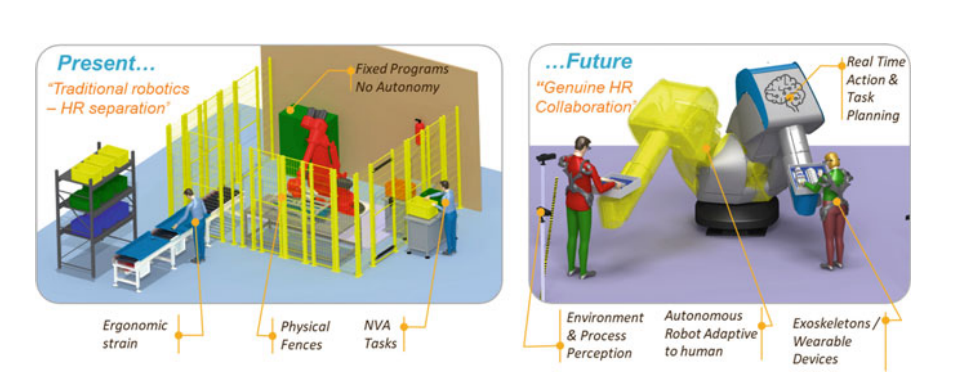
\includegraphics[width=1\linewidth]{Figures/Present and Future.png}
     \caption{Present and future of Industrial Human Robot collaboration\cite{author3}}
     \label{fig:2}
 \end{figure}
The types of human robot collaborations are explained in this chapter.
The authors also explain the current state of the standards and specifications for safe industrial robots in this article.This chapter also do a Qualitative comparison between industrial robots and human operator attributes. In this article the authors are pointing out the step changes to achieve true HRC.

These are

"1.Development of safety related technologies that will allow industrial robots to operate in fenceless environments and/or robots that are intrinsically safe to operate around humans.

2. Deployment of appropriate robotic systems depending on the requirements of the production environments (fixed high payload robots, mobile manipulators, drones, exoskeletons). 

3. Integration of Human Centred Interfaces which allow direct, natural and efficient ‘human to robot’ and ‘robot to human’ communication. The interface should be “invisible” during the interaction with the humans and ensure that physiological aspects are not negatively compromised.

4. Enablement of robotic perception to enable awareness of the tasks, environment and humans and cognition capabilities that allow them to reason upon the perceived states and adjust their behaviour for balancing task execution and interaction efficiency as a human operator would do."\cite{author3}
 
The authors points outlook on how HRC systems are expected to evolve and which are the key enablers for an efficient and sustainable uptake of this technology.
"The review has covered attempts to enable traditional robotic systems to act in a collaborative way as well as the conception and development of robots that are particularly built for the purpose. Although great leaps have been observed in individual technologies such as robotic cognition, machine vision, interfaces etc. there is still a lot of ground to be covered before seamless human robot collaboration can be achieved. From the industrial perspective and considering the technological state presented"\cite{author3}

In\cite{author4} the authors are pointing out various types of collaborative robots, manipulators and mobile, which are used in industrial environments. The authors also presents various industrial applications in which the robots are used in the industry, both in warehouse and inline production. The safety concerns are addressed in this. The introduction of sensors as precautionary methods and effectiveness of it is also discussed in this. The authors claim that the introduction of large number of the robots and the improved technologies like sensor vision, Artificial intelligence, Internet of Things enabled the 4th Industrial revolution.

In \cite{author5} The authors point out the shortcomings of the normative standards such as ISO/TS 15066 and proposes risk assessment approach resulting in a risk priority list. The author proposes FMEA and PRAT as techniques for risk assessment. A case study of robot employed for construction of brick-built residential units´and help masons is done. The proposed  eight steps are done on this . The eight stages proposed are Task branching,Hazard list,Body areas involved, Hazard categorization and Severity estimation, Interviews, Judgement description check, RPM computation and ranking, Risk priority list. The authors conclude after their case study that the robot cell is developed in a safe way, though the improvements for safety can be found out. This paper sets out an example for how to do risk assessment on the collaborative robot applications. Also the results of PRAT was compared with FMEA extensively used in HRC context, which are done by two different teams. 

In\cite{author6} the authors posits the HRC in manufacturing application increased the task performance ,by reducing completion time and minimizing error. An extensive review of literature was done in this article how HRC is contributing to the economic motivations, occupational health and efficient use of factory space. The authors suggest about the usage of traditional industrial robots in collaborative applications , to make use of high power of these robots. The authors discuss on the trends and future perspective of the HRC, the task of the robots in collaborative environments, the major industries in which the robots are used as the collaborative workers. Also the future trends of the market. The authors identify that since high product flexibility is possible with collaborative robots, also as the cobots are becoming cheaper in future SMEs may widely adopt cobots for wide range of industrial application.

In\cite{author7} the authors presents the advances in artificial intelligence in collaborative robots enables the robot to act in unstructured scenarios and interacting with unskilled and under trained users. Though the cobots are intrinsically safe, external sensing strategies improves safety.  The research trends on increasing perception of both human and robot are addressed in this article. The standards ISO 10128 part 1 and part 2 are reviewed , the technical specification ISO/TS 15066 is also reviewed. The upcoming revision of ISO 10128 is also addressed in this review. The most relevant standards dealing with safety requirements in HRC. is listed in this article. 

The ISO 691-4: 2020 provides some procedures for testing the driver-less industrial trucks designed to work automatically. This includes mobile robots in industry. The article also addresses the gaps in safety of robotic manipulators because of faster innovations and slower standardisation. The authors points out the testing and validation of  safety skill required for the robot.This includes validating of safety skills like maintain safe distance, maintain dynamic stability, limit physical interaction energy, limit range of movement, maintain proper alignment, limiting restrain energy.

 The authors of \cite{author8} raises their views on next generation robots , the evolution of an Human-Robot society and the categories of them, which would be there in near future are listed as industrial robots flexible for wide range of products and service robots which are capable of performing different tasks. The article raises queries about autonomy of the next generation robots and the safety issues, also about robot sociability problems. The authors point out role of AI in enabling autonomy for the robots.

 The authors view about the safety standards for next generation robots are interesting in a researchers point of view for formulating the safety standards on AI integration in robotics. The article states that the difference between traditional industrial robots and next generation robots in the safety standards is that first involves machine standards and the second involves machine standards and risk from unpredictable interactions in unstructured environments. The authors posits that the ISO 10128:2011 and the set of industrial standards addresses on the safety related parts of the control systems and the software and focuses on the robot arms and manipulator, these standards have limited application on next generation robots. Quoting the article "Complex Next Generation Robots motions, multi object interactions, and responses to shifts in environments resulting from complex interactions with humans cannot be reduced to simple performance parameters. Next Generation Robots and future Human-Based Intelligence designers and manufacturers must instead deal with unpredictable hazards associated with the legal concepts of core meaning and open texture risk."\cite{author8}.
 
 The artificial intelligence integrated robots will require a mix of pre safety and post safety mechanisms, the AI reasoning can be made for pre-safety. Safety intelligence , a system of artificial intelligence restrictions ,whose sole purpose is to provide safety when semi autonomous robot perform their tasks.So the human operator can always limit the robot autonomy. The authors suggests for clear and explicit design patterns so that semi autonomous robot can take protective reactions in human predictable ways to mitigate risks from unstable autonomous behaviour. An explicit interaction rule set and a legal architecture that can be applied to all kinds of Next Generation Robots.Also dynamic assessment of dynamic situations for response is suggested.
 
 \subsection{\RaggedRight Research on ISO/IEC Standards}{\normalfont\fontsize{14}{16}\bfseries} % Set section heading to 14pt

 In this section of the literature research on ISO 10128:2011 part 1 and part 2, ISO/TS 15066, ISO /IEC 23894 ,EN IEC 60812 are done . When first two listed standards are for the traditional industrial robots, the 3rd standard is for the risk assessment of AI integration in different systems. IEC 60812 to provide guidelines to perform Failure Mode Effective Analysis.

 Autonomous Driving is a parallel technology which can be viewed and how safety standards are implemented in the automobile software for Autonomous driving. In \cite{author9} the authors try to assess the adherence of the framework for Autonomous driving which is already in industry to ISO 26262. A case study was done on Apollo an Industrial Framework for Autonomous Driving. The observations from this article points to the need of standardisation and guidelines for GPU (Graphic processing Units) programming, which is now extensively used in processing AI algorithms.  In this paper the assessment is done and the complexities and missing features are found out and some recommendations are made for adhering the autonomous driving to ISO 26262.

EN ISO 10218:2011 which is the standard for the safe use of Industrial Robots has two parts. The first part EN ISO 10218-1 :2011" specifies the requirements and guidelines for the inherent safe design protective measures and information for use of industrial robots"\cite{author2} EN ISO 10218:2011 is harmonised standard for the European Union based on EN ISO 10218 and is approved by EUROPEAN COMMITTEE FOR STANDARDIZATION (CEN). In the endorsement it is written that CEN approved the ISO 10218-1:2011 without any modification. The standard does not address the robot as a complete machine, also the standard is not applicable for non industrial robots. There are some indispensable standards for the application of this standard which are mentioned in the section Normative reference of this standard. The basic terms and definitions of these terms are explained in the clause 3 of the standard.The Hazard identification and risk assessment is the content of the 4th clause which is based on ISO 12100. There is a list of hazards that can be present in with the robots in the Annex A of the standard, further hazard identification should be done and and risk assessment based on the identified hazards should be given particular consideration. Risk should be reduced or eliminated for particular scenarios like intended operation, unexpected startup, access for operators, foreseeable misuse of the robot, failure in the control system, and hazards associated with specific robot applications. 
 
 The design requirements in clause 5 of the standard are based on these identified risks. These requirements are made for the safe use of the manipulator or robot arm and the design of the control system in compliance with IEC 62061:2005 or ISO 13849-1:2006. In section 10 of clause 5 there are some guidelines for the collaborative operation requirements. The stopping conditions for the robot in collaborative operations are described in this.  The stop categories are in compliance with the standards IEC 60204-1. Clause 6 gives the verification and validation of the safety design and protective measures. The review of task-based risk assessment is interesting from a research point of view. 7th clause is about the information on the use of the robot. There are six annexes for the standard Annex A is already mentioned, Annex B for calculating safe distance for safeguard stop, and Annex C gives information about three position-enabling device and its functional characteristics. Annex D gives guidelines for optional features like Stopping performance measurement, mode selection, etc. Annex E gives guidelines for labeling and Annex 6 as guidelines for the verification of safety requirements and measures.

 Part 2 of ISO 10128,ISO 10128-2:2011, is made for the "recognition of the particular hazards that are presented in industrial robots when integrated and installed in industrial robot cells and lines"\cite{author10} This standard is also harmonised as EN ISO 10128-2:2011 and harmonization was without any modification by CEN.
 \begin{figure}[H]
     \centering
     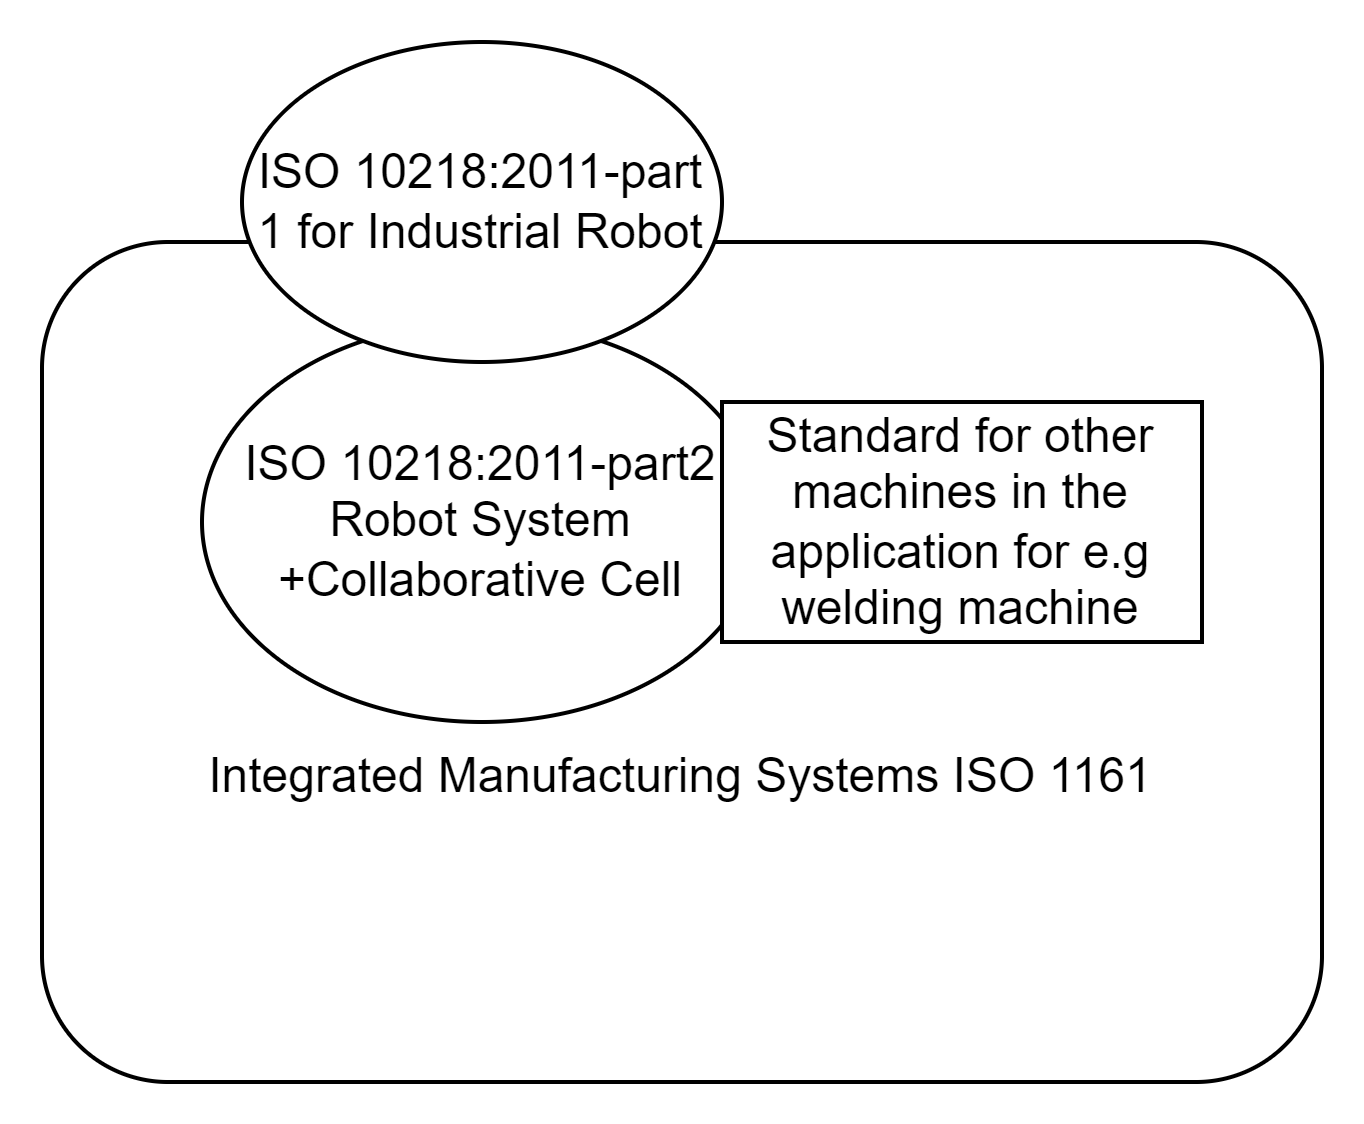
\includegraphics[width=0.5\linewidth]
   {Figures/Standard.png}
     \caption{Graphical view of relationships between standards\cite{author10}}
     \label{fig:2}
 \end{figure}

 In the normative reference of this standard, the standards for rules and safety of different power modes and layout of the workplaces are mentioned. Clause 4 is important since it gives guidelines for Hazard identification and risk assessment when the robot is integrated into a cell. The guidelines for layout design are also mentioned in this clause. The Hazard identification guideline in this standard is based on ISO 12100 and since this is particularly for robot systems. The guidelines for task identification and assessing hazardous situations that could arise from a particular task are very useful from a research point of view. The basic design of collaborative work spaces for traditional robots is also defined in clause 5 of this standard. The Annex E of the standard describes the conceptual applications of collaborative robots, which also describes safeguards for autonomous automatic operation within a common workspace.

 ISO/TS 15066:2016 \cite{author11} is the technical specifications required for industrial robots for safe collaborative applications, Hazard identification, and requirements for collaborative robot operations. The conditions for the operator to enter the collaborative workspace are specified and the power and force limiting specifications are defined. Annex A describes the Limits for quasi-static and transient contact. Maximum pressure values for quasi-static and transient contact between persons and the robot system are specified for each body part. The relationship between transferred energy and robot speed during transient contact is also mentioned in the Annex. 
 
Even if AI is integrated into robots the movement of the robot would be based on the control systems. The control systems may take input from the outputs of the AI Algorithm. If the control system is developed according to these standards and specifications the hazards can be limited.

The ISO /IEC standard for Information Technology -Artificial Intelligence -Guidance on risk management "gives guidance on how organizations that develop, produce, deploy or use products, systems, and services that utilize artificial intelligence (AI) can manage risk specifically related to AI."\cite{author12} This standard in its clause 4  states the principles of AI risk management. Risk management of systems should consider the whole system. AI systems can introduce new or emergent risks. Risk management principles, frameworks, and processes to tackle this is provided in this standard.
Various risk management principles applied to AI in compliance with ISO 31000 are stated in the standard. The standard gives guidance for Risk management processes. Guidelines on risk analysis are also presented in this standard. Annex B of the standard states the sources of risk, these sources must considered when risk is analysed. These are the Complexity of the environment, Lack of transparency and explainability, Level of Automation, Risk sources related to machine learning, System hardware issues, System life cycle issues, and Technology readiness. The ISO/ IEC 23894 also refers to ISO /IEC TR 5469, which is a technical report under process for functional safety in AI systems. The International Organisation for Standardisation realizes that AI systems can introduce new safety threats thus specific standards for particular application domains should be taken into account. Annex A of the standard also mentions the seriousness of the security requirement, since data poisoning and data stealing is possible. The standard also refers to ISO / IEC 22989 which is used for establishing terminology for AI and describes concepts in the field of AI.
The standard gives overall guidance for risk management of AI systems and also points to different standards that can be used for this. For, example ISO /IEC TR 24027 is a technical report on the bias and fairness of AI systems. ISO / IEC 24029-1 for robustness of neural networks. The information from this standard is very useful for doing risk assessment for AI.


EVS-EN IEC 60812:2018\cite{author13} is a standard that explains how failure modes and effect analysis are planned, performed, documented, and maintained. "The failure mode effects and analysis is to establish how items or process might fail to perform their function so that any required treatments could be identified."\cite{author13} This standard is a generic one, this is not giving any specific applications. The basic terms and abbreviations are specified in this standard. The purposes and objectives, the roles of persons, and the skill competencies of the persons involved in the analysis are defined. The methodology is explained from planning to documentation of the process with all the guidance for the analysis. The risk priority number based on the severity occurrence and detectability of the failure is a method of assigning criticality, there are other methods mentioned for the measurement of the criticality. The standard also includes some examples of FMEA from industry applications. The standard explains the procedure and application considerations for software and processes. Annex E describes in detail the consideration for software FMEA, and the examples of failure modes are described. The other important examples given are for system-level failure causes and programming errors. The generally used columns in the spreadsheet for software FMEA are also listed in this standard.
For process FMEA the starting point is a breakdown of the processes into steps. The flow diagram of the process should be analyzed.  The intended outcome of each step should be defined with a sufficient description of the specific function. The standard also describes the procedure for FMEA in planning safety applications. In addition, the standard also details safety-related control systems , which can diagnose internal failures online. Before the process, FMEA was used to analyze the manufacturing process, but now it is being used in every kind of process. 





 \subsection{\RaggedRight Research on Perception and AI based Grasping }{\normalfont\fontsize{14}{16}\bfseries} % Set section heading to 14pt

The motivation for doing research on perception and AI-based grasping is to study different algorithms, their unpredictability, identification of hazards, and analysis of risk. The growing significance of perception in human-robot interaction, makes robots flexible and adaptive enough for market demands.

\cite{author15} presents a comprehensive survey on robotic grasping using computer vision. Three key tasks in grasping is object localization, object pose estimation, and grasp estimation. The explanation for object localization is given as finding the potential regions of the target objects without categorizing them. Object detection outputs the bounding boxes for the identified objects according to their categories. Object instance segmentation provides further details as pixel level or point level regions of the target. The object localization can be based on the 2D or 3D inputs and this can be fitting 2D shape primitives when the object is viewed from a fixed angle. In 2D salient object classification the arbitrary shapes are output to the detected objects.
3D localization without classification deals with 3D point cloud input, similar to 2D object localization there are 2 types described for 3D also, which are Fitting 3D shape primitives and 3D salient object detection. The shape primitives are mostly box, cylinders, or spheres. The 3D salient object detection uses RGB-D camera for depth analysis also uses fused data from the sensors for object localization. Object detection can be explained as the localization of the objects along with the classification of individual objects using a two-stage method or one-stage method. Similarly, the object instance gives the output as a detailed point cloud.
Object pose estimation means finding out the 2d position and in-plane rotation angle for 2D planar grasps and 3D position and 3D orientation of the object. 6D object pose estimation is found out by transforming the object coordinate to the camera coordinate.
For object pose estimation there are 3 methods described in this paper. 
1) Correspondence-based methods, which is again subdivided into  2D image-based methods and 3D point cloud-based methods. In the 2D image-based method the correspondence is established through matching outputs from the RGB camera and the rendered 3D point.in 3D point cloud-based methods the correspondence is established by 3D point cloud from the RGB-D point cloud and the 3D geometric descriptors.
2) Template-based methods, involve comparison of the labeled with Ground Truth 6D object poses with obtained template.
3) Voting-based methods are further classified into Indirect voting methods and Direct voting methods. Each pixel or voxel points vote for some feature points on the correspondences.
Grasp estimation means finding out the 6D pose of the gripper concerning the camera coordinate. There are 2D planar grasp and 6 DoF grasp. In a 2D planar grasp, the grasp is constrained from one direction, thus the grasp contact points can define the gripper's grasp pose. Force analytic and object geometry is important in grasp estimation, but there is only limited data for the empirical methods of grasping causing troubles when unknown objects are being grasped. The grasp qualities are measured using Grasp quality -CNN network. In 6 DoF grasp methods are based on the point clouds and the complete shape. For 6 DoF grasp, there are different methods, methods estimating grasp qualities of candidate grasps and methods of transferring grasps from existing ones.
The conclusion of the paper states the challenges, such as insufficient information in data acquisition, an insufficient amount of training data, a generalized approach in grasping novel objects, and challenges from grasping transparent objects. The adoption of multi-view data and multi-sensor data including data from haptic sensors. For tackling insufficient amounts of data the simulation environment can be built. Usage of semi-supervised learning and self-supervised learning methods to generate labeled data for 6D object pose estimation. Using plenoptic sensing.

In \cite{author16} the authors are assessing the Human-Robot perception in industrial environments. Different types of devices used for perception, especially RGB-D Camera, and the algorithms used for the functioning of these sensors along with the robot are also reviewed. The usage of these sensors in different types of robots like, fixed manipulators and mobile manipulators are also reviewed. The authors consider two scenarios of HRC with fixed manipulators. Robots have full awareness of the presence of humans. Only the awareness of the shared spaces can be sufficient, guaranteeing no human can be hurt while the robot is in motion. The usages of proprioceptive-based methods and exteroceptive methods for enhancing HRC are also reviewed. The accuracy and repetitiveness of the exteroceptive methods are still to be improved. The type of sensor, the methodology to use the sensor and the results of the methodology are the authors' interest of research. the authors made it clear that when sensor accuracy is less, the complexity of algorithms aims for compensation, to achieve an overall reliable interaction. The authors conclude based on the research that. Vision sensors are fundamental for detecting human presence in robotic systems. The data from sensor fusion can be helpful for new types of collaboration and applications. Laser sensors are also used in robotic systems in combination with vision ones mostly in the case of mobile robots. The authors also find out that, the use of non-standard sensors is still limited. 

In the report "Toward Safe Perception in Human-Robot Interaction" \cite{author17} the authors states perception as an important component of safety in Human-Robot Interaction. A safe mechanical design of the robot may reduce the potential hazards, but to have a detailed knowledge of the surroundings and the state of the robot and the human operator is much beneficiary. The report suggests requirements for a holistic architecture to construct safe perception. The authors suggests the redesigning of the system is the most effective risk reduction strategy, but in less structured environment when operating adaptively redesigning alone is insufficient in most cases. To overcome this shortcoming combining of the other approaches like functional or physical safeguards and raising the awareness of the operator or user is also proposed. The report posits the use of multiple sensors and fusion of data from these sensors for redundancy. The report gives an overview about how to proceed risk analysis in safe perception. which would be very much useful from research point of view. Also suggests an architecture for safe perception for a typical collaborative robot based on the risk assessment.The usage of highly dependable sensors for perception ,at performance level D for human collaboration, for environmental perception the ToF cameras are suggested.High redundancy and heterogeneous sensors is considered as a pre-requisite for fulfilling the safety requirements. 

In\cite{author18} the authors are presenting the failure modes of robotic bin picking induced from perception uncertainties. The human intervention is invoked when the robot fails . The paper describes the importance of the bin picking application using the industrial robots, since it offers a flexible automation solution. The paper explains how the complexity of bin picking increases as the shape complexity increases. Uncertainties in locating the part and the orientation of the part also leads to failure. The other perception uncertainties induced from potential of the parts for getting tangled and occlusion of grasping surfaces makes the planning challenging. Mainly the perception uncertainty leads to detection failure or singulation planning failure. The authors also give review about the related works in which uncertainties of the force, friction and contact location for grasp. The authors state they are interested in measuring the performance as a composite of "1) quality off approach of toward the object2) grasp quality, and 3) quality of extraction of the grasped object"[18]. The paper also illustrates the confidence assessment of the robot to complete a task, so that failure of the system can be prevented, hazards and lose of money from system shutdown from these failures can also be stopped. The authors present an approach that sees uncertainty as key to the failure of bin picking and suggests methods to deal with it.

In \cite{author19} the authors try to demonstrate a framework which would take into account  the overall probability of success of each grasp taking into account the error from incorrect object detection and motion error due to imperfect robot calibration. This framework takes input from multiple object detectors, grasp planners and grasp evaluators and combines these interpretations. Then uses a Bayes net model to evaluate success of each grasp. This approach can be used as a  procedure for avoiding uncertainty in grasping.

In \cite{author20} the authors aim to present perception challenges for grasping in clutter and unpredictable relative motion between robot and object. The authors review different types of grasping perception systems in this work. The authors investigate on performance benefits of dynamic grasping of a perception system designed to prevail the disadvantages due to occlusion, limited field of view, and minimum sensor range of a traditional wrist camera. the authors conclude stating that the placement of the perception systems is very crucial part in designing a robust robotics system. This research is focused on mobile manipulators and dynamic environment , where the manipulator and the work piece might be having high relative motion. The inputs from the research could be taken and can be upgraded, mainly about the placement of the camera, since in the company we have MAiRa Robot, which has the camera integrated in the industrial arm, and is suitable for the grasping in dynamic environment. 

\cite{author21} is a summary of the research challenges and Progress in Robotic grasping and Manipulation competition by IEEE Robotics and Automation Magazine. Different challenges in vision based grasping is addressed in this paper. The challenges faced in mechanism level, algorithm level and system level by the competitors are addressed. The authors tried to show the recent advancements in tackling this challenges and progress made by engineering. Also progress made by introduction of advanced hardware is also explained in this paper. The Aim of this competition is to to analyse the future research directions.The paper also gives references to benchmarks for assessment of the robustness and resilience of the mechanism. Also references for evaluation of performance of the Algorithm and Task performance by the system.
The paper projects the major challenges in perception as identifying the objects with shiny surfaces, objects that are translucent and tasks which need high level of precision and accuracy. Challenges in grasping mechanisms are , grasping with imperfect perception, since perception errors are the reason for most of the grasping failures. For example if the object's pose is not correctly identified the robot could knock over or push away the object and then improper grasping could happen.Since noise from the sensor outputs is present always the concept of perfect perception is almost impossible.Other challenges in grasping is picking up objects with complex shapes and grasping objects from clutter . Re-grasping is a major challenge since the objects needed to be adjusted after initial grasp in many of the applications.The paper also presents grasping for manipulation and in hand manipulation as very challenging areas.The authors also try to present the challenges in manipulation. 
The paper is concluded by pointing out, how the tasks which were considered tough, is now being solved using different approaches. Also by sharing the future scopes and ongoing researches on vision based grasp for robots.
 The authors in \cite{author22} tries to implement bench-marking for grasp planning algorithms. It is a very complex process since numerous factors that are diverse and complex are involved in this. The main challenges are the evaluation of grasp planning algorithm based on the influence of vision system and the arm independently.Other challenges include the difficulties confounded when doing the experiments. 
 Lack of principle methodology that clearly defines steps in the grasping pipeline also is an issue. Standardizing this is also a major concern.The method for comparing performance of different grasp planning algorithms which can be applied for model based and model free approaches is presented in this paper. The paper presents an empirical method of verification and validation of different grasp algorithms , it explains the robot set up, the environment and the method for this verification. This method can be used to validate the algorithm , when known objects are being picked in known environments. To find out the unknown incidents that can happen in unpredictable times this method is not recommended. 
GRASPA 1.0 explained in \cite{author23}is a robotic grasping performance bench-marking.In this paper the environment for the benchmark is defined. Reachability within the layout camera calibration within the layout and  graspability according to the maximum payloads for different robots grasp quality, execution and stability of the grasp are considered for considering the score for benchmark.

 \subsection{\RaggedRight Perception in Robotics: Risk Assessment Methods from Autonomous Driving Systems}{\normalfont\fontsize{14}{16}\bfseries} % Set section heading to 14pt

Autonomous Driving systems have more complex perception than collaborative robots since the environment for the robot is limited and more predictable than the vehicle. The stringent risk assessment methods used in AD and the safety framework can be adapted for robots.
When perception-based grasping alone is considered its low-level autonomy and the sensor performance and the algorithm's performance requirement are relatively low, when medium-level autonomy, which means robots do object identification and grasping along with collision avoidance and human detection the requirements of the algorithm are relatively high. 

In \cite{author24} the authors discuss the safety of perception systems in autonomous driving systems. The progress in the standardization, research advances and perspectives is also discussed. The authors are concerned about challenges in perception due to the operational conditions the edge cases and the requirements and problems of human monitoring and intervention. One of the core issues pointed out by the authors is the reliability of the black box perception systems which is outlined in the Safety of the Intended functionalities. (SOTIF). The authors also explain the main failures in perception tasks. In object detection, the two most common failures are False positives and False Negatives. False positive (FP) occurs when the object detection algorithm identifies a nonexisting object in the environment by mistake. False negatives (FN) may occur when the algorithm fails to identify an existing object in the environment. The failures occurring in object tracking can be losing track of an object due to occlusion, switching track to another object, and object re-identification. Over or under-segmentation of the scene is the most commonly occurring segmentation fault. For Autonomous Driving Systems (ADS) predictions of the object behavior are important and the failures include inaccurate predictions or missed predictions. The authors also explain the necessity of a clear framework for the development and deployment of perception systems.  There are arguments stated in the paper about the perception that should address safety requirements for all ASIL attributes. ISO 21488 is further proposed for functional safety during system failures as perception systems have functional insufficiency. The standards like ANSI/UL 4600 for the safety and performance of autonomous products. The ontology for ADS  taxonomy and standards describes 
 When it is safe for ADS and How to demonstrate system safety: based on the operating road conditions, traffic volume weather conditions, and the working state of the vehicle.
The paper also explains the cause-effect chain for the intended functionality of perception, sensing, and inference which can be further used in sensor failure mitigation and sensor fusion research. Also, this helps in a challenging but very important step, quantifying the complex data-driven system's level of safety. High-fidelity models for high-level perception systems can generate realistic results but the computational power required limits the real-time capability. the black box model to describe sensing and inference at the same time is another trend. It tries to find a direct association between final failures and the scenario. Parametrization of perception uncertainty is a goal to achieve in the future. The paper also describes the measurement of perception safety. Traditional offline safety metrics evaluate sensor inputs and outputs of ADS. Which is largely based on the ability to detect the FNs and FPs. Uncertainty estimation is important in measuring perception safety in real-time which is based on the soft-max function as explained in the paper. This helps in providing early warnings for perception hazards. The uncertainty provides an estimate of how confident the prediction is, but they still lack any reference to real ground truth. Redundancy measures and evidence checks are used. Redundant information can be taken from different sources a pre-defined model can be used and real-time data can be cross-verified with this pre-defined model. Cooperative perception is now the trending research subject for increasing safety as per the authors. The basic idea presented is an information fusion scheme, thus increasing accuracy and reducing uncertainty. early fusion, intermediate fusion, and late fusion are implemented to achieve robust results. The authors claim that even though many cooperative perception models are being made there are new dimensions of safety concerns. This includes safety regarding communication infrastructure, local dependencies, and network-related issues. The authors also explain the V2I and V2X connection for information sharing which should be secure, for improved cooperative perception, this also can reduce edge computing nodes.
The research scope of Explainable AI also sheds light on the trustable performance of the machine even when the AI model fails and is considered in the future scope of the research.

Evaluation of the safety of intended functionality is highly essential.\cite{author25} presents a concept for this. As per the authors of \cite{author25} the safety of the intended functionality is important because of the potential hazards due to the limitation of the design and implementation of the perception algorithms, and hardware performance, in SOTIF norms the limitations described are particular to the components with neural networks. In the Automotive industry, the SOTIF analysis helps in how to create or generate test cases systematically.[25] gives a contribution to evaluating the safety level of perception of the automotive system. The safety goal presented in this paper is to reduce unknown unsafe incidents and to reduce known unsafe scenarios. The authors state that risk can be calculated as the product of severity and probability, in which severity is a deterministic parameter. Probability should be found using statistical analysis. The steps like System error recovery, Partition of system failures Modelling of hazardous events, and Analysis of traffic statics are done to define test scenarios.

In \cite{author26}the authors performed an analysis of how safe work can be done by an autonomous guided vehicle in a logistic environment, using SOTIF. Figure  4 shows the reduction in risks and the type of risks being reduced before and after the SOTIF analysis.

\begin{figure}
    \centering
    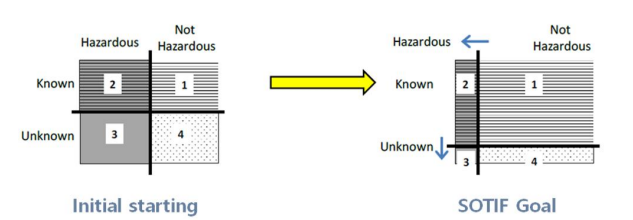
\includegraphics[width=0.7\linewidth]{Figures/The goal of SOTIF Analysis.png}
    \caption{The goal of SOTIF Analysis \cite{author26}}
    \label{fig:enter-label}
\end{figure}

Area 3 in Figure 4 represents the unknown risks, the goal of SOTIF is to reduce Area 2 and Area 3 in the graph. These are not because of the failure but because of the impact of the surrounding environment, and limitations of situational perception according to technology performance. The authors suggest the usage of SOTIF to prevent accidents due to wrong perception or wrong performance evaluation of the algorithm in certain situations. Responsibility Sensitive Safety model based on the camera sensors is also trending in current research topics. The task of the mobile robot should be identified in a pre-requirement stage. The safety specifications should be designed according to the safety requirements identified in addition to general safety requirements. The authors present the errors and the identified hazards in this paper for the Autonomous driving logistics robot. The paper presents a flowchart of the SOTIF process applied for the automated guided vehicle which we can try to integrate in case of robots making use of AI. The paper also presents what each clause of the SOTIF is addressing and how it was used for AGVs. The authors claim by applying the SOTIF methodology risks that can occur are eliminated as much as possible. They propose using the RSS model and SOTIF for the Design application of AGV.

In \cite{author27} the authors review and organize practical machine learning techniques that complement to the engineering safety for machine learning-based software in autonomous vehicles. the authors suggest the iterative risk assessment for the autonomous software to formally represent the operational design domain. The authors posit that the prediction probability scores in Deep Neural Networks do not provide the correct model of the uncertainty. Security challenges are there since the DNNs can be attacked and any input data alteration can fool a DNN. the paper studies ISO 26262 and ISO/PAS 21448 Standards for the Automotive vehicle. Since ISO 26262 cannot account for the faults occurring due to the the inability of the component to comprehend the environment. The authors states around 40 percentage of the software safety methods from ISO 26262 do not apply to the ML models. The Design specification is not enough for the software of the ML model because the model try to target the classes not any specification.Implementation of transparency which is specified in ISO 26262 is also not possible in ML models since ML is using high dimensional data. Testing and validation of the software is highly recommended in ISO 26262 to enforce there is no dead or unreachable code, for DNNs formally specifying their correctness is challenging. SOTIF standards  treats the ML models as black box and learning problems would be there because of the error in the learning model. Run time monitoring also is an important factor that is difficult to achieve in DNN and many other machine learning models. The techniques for ML safety is stated in this paper. These techniques compliment the classic engineering  strategies in software safety. To reach inherently safe AI the mankind has to travel more far. Safe fail and Safety margins must be defined. One of the practical ML safety solutions is to monitor the misclassification error detection to achieve fail safe. A parallel error detection unit should be working to monitor the transient error inputs from the hardware.Also run time monitors should be designed three of them are listed by the authors 

Uncertainty Estimation, quantifying uncertainty can explain what a model does not know in terms of model confidence on its prediction.The computation cost and hardware requirement is a challenge in this.
In-Distribution Error Detectors, due to weak representation learning misclassification of in domain samples often happens, large training data sets improved DNN . Selective classification is a technique to provide high confidence samples.

Out of Distribution Error Detectors, OOD samples are the samples that are outside of the normal training distribution. OOD error is an inherent problem, revision of network architecture for learning the prediction confidence and self supervised approaches for outlier detection. Improving the algorithm's robustness is one of the the methods suggested for monitoring the machine learning algorithm. the authors propose Robustness to domain shift and Robustness to corruptions and perturbations. Robustness to Domain shift, Domain is the variations in the input data set compared to the training set. this reduces the performance, to overcome this domain generalization is important, unsupervised learning. Robustness to Corruptions and perturbations, data correction, and perturbation exist in the open world. Achieving model robustness to natural corruption is to improve model robustness above their clean data set.

The acceptance criteria and validation target are explained in \cite{author28} for ADS. The factors for acceptance criteria are listed as ODD factors and their attributes, Driver characteristics, Statistical factors, Relevance of Database and Values, Derivable Data, type of Rationale, possibility of multiple values, Distance vs Time, and Recentness of Data. Factors to consider for validation target are listed as Confidence level, Safety Margin, Distribution among simulation vs real-world testing, Scenario Coverage, and Multiple Acceptance Criteria, Also the authors illustrate examples in the paper for better understanding. A comprehensive results are also provided in the conclusion which we can adapt to the situations applicable to robots.

\cite{author28} suggests techniques for uncertainty evaluation in the object detection algorithms for Autonomous Vehicles.Different techniques like confusion matrix, precision-recall curve, receiver operating curve´, and F-score matrix are all used in the evaluation of image classification models. The authors also suggest SOTIF analysis for the developers to test and compare the performance of the networks. The authors explain a case study for the uncertainty evaluation. 

\subsection{\RaggedRight Risk Assessment with FMEA in Industry 4.0}{\normalfont\fontsize{14}{16}\bfseries} % Set section heading to 14pt
In \cite{author14} the authors propose FMEA-AI which is a modification for FMEA. The proposed method helps to identify safety and fairness risks in multiple failure modes of an AI system. The paper portrays "impact assessment" as an emerging mechanism to regulate AI systems. Also, the authors state that in the past AI was linked with Failure mode analysis focused on applying machine learning methods to autonomously perform FMEA, but there was no definition for identifying ways in which AI might fail. As per the author, FMEA has become a safety symbol of functional safety. The article provides two examples of doing FMEA-AI in which one is an analysis of potential applications for visual detection systems and the other one is an analysis of a series of failure modes for a single AI application. The context of severity and unfairness is explained in this article by the authors. In the proposed method people are divided into user groups to find out the unfairness. The article gives an outlook on how the probability of occurrence, risk, and mitigation is considered. The FMEA work sheet for a specific application can be used as a guideline for doing FMEA on the application AI-based perception and grasping.

In\cite{author30} the authors propose FMEA-STPA for risk analysis in intelligent and collaborative automation systems. Since this is predicted to be an important part of flexible manufacturing. This could contribute to evaluating the architectural design, and the risks and applying the risk reduction measures. While FMEA contributes to the system through reliability theory STPA contributes through system thinking. The authors explore the integration of FMEA and STPA to address the challenges that arise from the gaps in the guidelines addressing risk related to machines empowered by AI. This allows a more holistic analysis of the control structure. The promising path opened by this integration of risk assessment tools a more comprehensive evaluation of safety is ensured. In this article the authors show how the risk assessment techniques from Autonomous systems of a car complement the robotic field. The previous papers published by the authors of this paper also suggest planned safety , and its implementation \cite{author35} which is also suggested in this thesis and use-case to avoid compromising the cycle times of the application.

\subsection{\RaggedRight Conclusions from the Literature Review}{\normalfont\fontsize{14}{16}\bfseries} % Set section heading to 14pt

The first part of the review gave ideas about the improvement of human-robot interactions using AI and how important the integration of AI in robotics is. The research on ISO/IEC Standards like EN ISO 10218-1,2:2011  gave light on the risks of robots in the industrial atmosphere. General standards like IEC 61508 and ISO 12100 gave ideas on determining the risk and methods to determine risk. The review of IEC 60812:2018 gave guidelines to do FMEA which helps to quantify risks. The ISO/TS 15066 also gives specifications for mitigating the risk of collaborative robots. The study of grasping algorithms could contribute to understanding how perception-based grasping is working and what can be the possible failures.
The research on the safety of perception systems of autonomous vehicles helped to contribute to understanding the failures from the algorithms also the techniques used to mitigate them. The knowledge gained from this literature review is used as the base for the methodology of the thesis.



 




